% Template per generare 

\documentclass[a4paper,11pt]{article}
\usepackage{lmodern}
\renewcommand*\familydefault{\sfdefault}
\usepackage{sfmath}
\usepackage[utf8]{inputenc}
\usepackage[T1]{fontenc}
\usepackage[italian]{babel}
\usepackage{indentfirst}
\usepackage{graphicx}
\usepackage{tikz}
\usepackage{listings}
\newcommand*\circled[1]{\tikz[baseline=(char.base)]{
		\node[shape=circle,draw,inner sep=2pt] (char) {#1};}}
\usepackage{enumitem}
% \usepackage[group-separator={\,}]{siunitx}
\usepackage[left=2cm, right=2cm, bottom=3cm]{geometry}
\frenchspacing

\newcommand{\num}[1]{#1}

% Macro varie...
\newcommand{\file}[1]{\texttt{#1}}
\renewcommand{\arraystretch}{1.3}
\newcommand{\esempio}[2]{
\noindent\begin{minipage}{\textwidth}
\begin{tabular}{|p{11cm}|p{5cm}|}
	\hline
      \textbf{\file{input (da stdin)}} & \textbf{\file{output (su stdout)}}\\
	\hline
	\tt \small #1 &
	\tt \small #2 \\
	\hline
\end{tabular}
\end{minipage}
}

% Dati del task
\newcommand{\gara}{IOI 2002}
\newcommand{\nome}{Specchio}
\newcommand{\nomebreve}{specchio}

\begin{document}
% Intestazione
\noindent{\Large \gara}
\vspace{0.5cm}

\noindent{\Huge \textbf \nome~(\texttt{\nomebreve})}

% Descrizione del task
\section*{Descrizione del problema}

Un \emph{albero (ordinato)} \`e formato da una \emph{radice} e da un insieme finito e ordinato (eventualmente vuoto) di \emph{figli}, che sono anch'essi alberi. Ad esempio, la Figura~1 rappresenta un albero: per convenzione, la radice viene disegnata in cima (cio\`e al contrario rispetto agli alberi veri). Come ogni albero, lo potete descrivere dicendo quanti figli ha la radice (in questo caso, $4$) e poi descrivendo uno a uno, nell'ordine da sinistra a destra, i $4$ sotto-alberi. In questo modo, ad esempio, l'albero in Figura~1 sarebbe identificato dalla seguente sequenza:
\[
4\,\,\,2\,\,\,0\,\,\,3\,\,\,0\,\,\,0\,\,\,1\,\,\,0\,\,\,0\,\,\,0\,\,\,0
\]	

\begin{figure}[h!]
  \centering
    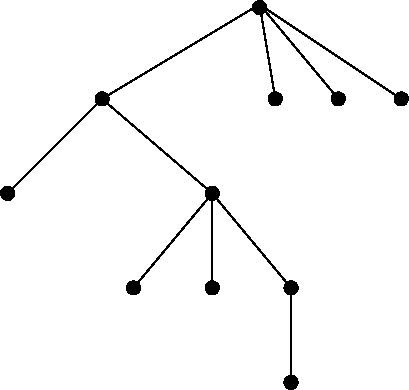
\includegraphics[scale=0.3]{figs/fig1.png}\\
    \caption{Un albero.}
\end{figure}

Infatti, l'albero ha quattro figli sotto la radice, per cui il primo numero \`e $4$. A questo $4$ segue poi subito la sequenza $2\,\,\,0\,\,\,3\,\,\,0\,\,\,0\,\,\,1\,\,\,0$, che \`e la descrizione del primo figlio, mentre gli ultimi tre figli sono ciascuno descritti da $0$ (dato che non hanno figli).

Supponete ora di guardare l'albero riflesso in uno specchio. L'ordine dei figli di ciascun nodo risulta invertito e l'albero di Figura~1 appare come in Figura~2.

\begin{figure}[h!]
  \centering
    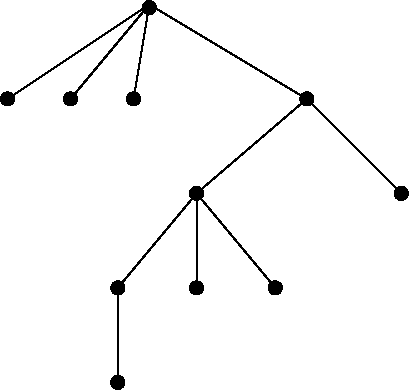
\includegraphics[scale=0.3]{figs/fig2.png}\\
    \caption{L'albero di Figura~1 allo specchio.}
\end{figure}

Questo nuovo albero \`e descritto dalla sequenza
\[
4\,\,\,0\,\,\,0\,\,\,0\,\,\,2\,\,\,3\,\,\,1\,\,\,0\,\,\,0\,\,\,0\,\,\,0
\]

Fornire un metodo per passare dalla descrizione di un albero alla descrizione del suo rovesciato sinistra-destra (e viceversa).


% Input
\section*{Dati di input}

La prima riga contiene $T$, il numero di testcase da risolvere. Seguono $T$
istanze del problema. Ogni istanza consta di una sola riga che codifica, come sopra spiegato, l'albero da rovesciare nello specchio.
In pratica, la riga contiene una sequenza di interi non negativi, separati da spazi. La sequenza descrive correttamente un albero: quindi il primo numero è il numero di figli della radice, ed è immediatamente seguito dalle descrizioni dei sotto-alberi radicati nei figli della radice, prese una dopo l'altra, nel loro ordine da sinistra a destra.

% Output
\section*{Dati di output}

L'output deve contenere una riga per ogni testase. Tale riga è costituita da una sequenza di interi non negativi separati da spazi. Tale sequenza è intesa codificare, secondo le stesse regole che per l'input già viste sopra, l'albero rovesciato sinistra-destra, ossia l'albero dato in input visto allo specchio.

% Esempi
\section*{Esempio di input/output}
\esempio{
4 2 0 3 0 0 1 0 0 0 0
}{
4 0 0 0 2 3 1 0 0 0 0
}

\esempio{
4 0 0 0 2 3 1 0 0 0 0
}{
4 2 0 3 0 0 1 0 0 0 0
}


% Subtasks
\section*{Subtask}

Il tempo limite per istanza (ossia per ciascun testcase) è sempre di $1$ secondo.

Per il subtasking sono previste le seguenti `size`:

\begin{description}
\item[\textbf{\hspace{1ex}[2 istanze] esempi\_testo:}] i due esempi del testo.
\item [\textbf{[21 istanze] small:}] $N \le 10$.
\item [\textbf{[22 istanze] medium:}] $N \le 100$.
\item [\textbf{[16 istanze] big\_binary:}] $N \le 100\,000$.
\item [\textbf{[16 istanze] big\_max\_2\_children:}] $N \le 100\,000$.
\item [\textbf{[23 istanze] big:}] $N \le 100\,000$.
\end{description}

In generale, quando si richiede la valutazione di un subtask vengono valutati anche i subtask che li precedono, ma si evita di avventurarsi in subtask successivi  fuori dalla portata del tuo programma che potrebbe andare in crash o comportare tempi lunghi per ottenere la valutazione completa della sottomissione. Ad esempio, chiamando:

\begin{verbatim}
    rtal -s wss://ta.di.univr.it/algo  connect -a size=medium  specchio -- python my_solution.py
\end{verbatim}

\noindent
vengono valutati, nell'ordine, i subtask:\\

{\tt esempi\_testo}, {\tt small}, {\tt medium}.\\

\noindent
Il valore di default per l'argomento {\tt size} è {\tt big} che include tutti i testcase.\\


\end{document}
